\documentclass[letterpaper]{article} % DO NOT CHANGE THIS
\usepackage[submission]{aaai2027}  % DO NOT CHANGE THIS
\usepackage[hyphens]{url}  % DO NOT CHANGE THIS
\usepackage{graphicx} % DO NOT CHANGE THIS
\urlstyle{rm} % DO NOT CHANGE THIS
\def\UrlFont{\rm}  % DO NOT CHANGE THIS
\usepackage{natbib}  % DO NOT CHANGE THIS AND DO NOT ADD ANY OPTIONS TO IT
\usepackage{caption} % DO NOT CHANGE THIS AND DO NOT ADD ANY OPTIONS TO IT
\frenchspacing  % DO NOT CHANGE THIS
\usepackage{booktabs}
\pdfinfo{
/TemplateVersion (2027.1)
}
\setcounter{secnumdepth}{2}

% Generated by analysis/make_tex.py; do not edit.
\newcommand{\nTestImages}{1{,}111}
\newcommand{\nTestObjects}{10{,}517}
\newcommand{\nSeaCucumber}{1{,}079}
\newcommand{\nSeaUrchin}{7{,}201}
\newcommand{\nScallop}{217}
\newcommand{\nStarfish}{2{,}020}
\newcommand{\shareSeaUrchin}{68}
\newcommand{\apYoloEightN}{0.624}
\newcommand{\ciYoloEightN}{[0.593, 0.655]}
\newcommand{\apYoloN}{0.625}
\newcommand{\ciYoloN}{[0.595, 0.652]}
\newcommand{\apYoloL}{0.690}
\newcommand{\ciYoloL}{[0.662, 0.716]}
\newcommand{\apGD}{0.090}
\newcommand{\ciGD}{[0.067, 0.114]}
\newcommand{\apGDtext}{0.048}
\newcommand{\ciGDtext}{[0.030, 0.069]}
\newcommand{\apOWL}{0.099}
\newcommand{\ciOWL}{[0.088, 0.111]}
\newcommand{\apQThree}{0.000}
\newcommand{\ciQThree}{[0.000, 0.000]}
\newcommand{\apQSeven}{0.013}
\newcommand{\ciQSeven}{[0.009, 0.018]}
\newcommand{\apGDlatin}{0.081}
\newcommand{\ciGDlatin}{[0.067, 0.100]}
\newcommand{\apOWLlatin}{0.086}
\newcommand{\ciOWLlatin}{[0.067, 0.105]}
\newcommand{\apQSevenLow}{0.007}
\newcommand{\ciQSevenLow}{[0.005, 0.015]}
\newcommand{\apQwenVL}{0.048}
\newcommand{\ciQwenVL}{[0.043, 0.056]}
\newcommand{\apHQwenVL}{0.054}
\newcommand{\ciHQwenVL}{[0.043, 0.087]}
\newcommand{\apHGD}{0.078}
\newcommand{\ciHGD}{[0.048, 0.138]}
\newcommand{\apHOWL}{0.107}
\newcommand{\ciHOWL}{[0.078, 0.140]}
\newcommand{\apHQSeven}{0.018}
\newcommand{\ciHQSeven}{[0.006, 0.034]}
\newcommand{\apHQThree}{0.000}
\newcommand{\ciHQThree}{[0.000, 0.000]}
\newcommand{\apHQSevenNoEmpty}{0.018}
\newcommand{\ciHQSevenNoEmpty}{[0.011, 0.030]}
\newcommand{\apHQThreeNoEmpty}{0.017}
\newcommand{\ciHQThreeNoEmpty}{[0.009, 0.032]}
\newcommand{\dGap}{+0.525}
\newcommand{\dciGap}{[0.493, 0.554]}
\newcommand{\dDecoding}{+0.042}
\newcommand{\dciDecoding}{[0.032, 0.053]}
\newcommand{\dOwlGd}{+0.009}
\newcommand{\dciOwlGd}{[$-$0.015, 0.031]}
\newcommand{\dLatinGd}{+0.009}
\newcommand{\dciLatinGd}{[$-$0.001, 0.016]}
\newcommand{\dLatinOwl}{+0.013}
\newcommand{\dciLatinOwl}{[0.001, 0.025]}
\newcommand{\dSevenThree}{+0.013}
\newcommand{\dciSevenThree}{[0.009, 0.018]}
\newcommand{\dResolution}{+0.005}
\newcommand{\dciResolution}{[$-$0.002, 0.009]}
\newcommand{\dYoloSize}{+0.065}
\newcommand{\dciYoloSize}{[0.056, 0.074]}
\newcommand{\dQwenGenFull}{+0.035}
\newcommand{\dciQwenGenFull}{[0.029, 0.043]}
\newcommand{\dOwlQwenFull}{+0.051}
\newcommand{\dciOwlQwenFull}{[0.040, 0.061]}
\newcommand{\dGdQwenFull}{+0.043}
\newcommand{\dciGdQwenFull}{[0.016, 0.064]}
\newcommand{\dQwenGen}{+0.036}
\newcommand{\dciQwenGen}{[0.021, 0.066]}
\newcommand{\dGdQwen}{+0.024}
\newcommand{\dciGdQwen}{[$-$0.014, 0.076]}
\newcommand{\dOwlQwen}{+0.053}
\newcommand{\dciOwlQwen}{[0.017, 0.078]}
\newcommand{\dPromptSeven}{+0.000}
\newcommand{\dciPromptSeven}{[$-$0.009, 0.011]}
\newcommand{\dPromptThree}{+0.017}
\newcommand{\dciPromptThree}{[0.009, 0.032]}
\newcommand{\rhoCocoDuo}{0.83}
\newcommand{\rhoCocoDuoCI}{[0.66, 0.94]}
\newcommand{\mgGD}{0.136}
\newcommand{\mgciGD}{[0.127, 0.146]}
\newcommand{\mgOWL}{0.151}
\newcommand{\mgciOWL}{[0.139, 0.164]}
\newcommand{\mgYoloN}{0.705}
\newcommand{\mgciYoloN}{[0.687, 0.725]}
\newcommand{\mgYoloL}{0.744}
\newcommand{\mgciYoloL}{[0.724, 0.763]}
\newcommand{\mgQSeven}{0.016}
\newcommand{\mgciQSeven}{[0.011, 0.019]}
\newcommand{\mgQwenVL}{0.083}
\newcommand{\mgciQwenVL}{[0.076, 0.094]}
\newcommand{\scApGD}{0.004}
\newcommand{\scApciGD}{[0.002, 0.008]}
\newcommand{\scApOWL}{0.001}
\newcommand{\scApciOWL}{[0.001, 0.002]}
\newcommand{\scApYoloN}{0.606}
\newcommand{\foundGD}{69}
\newcommand{\namedGD}{59}
\newcommand{\foundciGD}{[67, 72]}
\newcommand{\namedciGD}{[57, 61]}
\newcommand{\scFoundGD}{61}
\newcommand{\scNamedGD}{4}
\newcommand{\scFoundciGD}{[57, 65]}
\newcommand{\scNamedciGD}{[3, 6]}
\newcommand{\foundOWL}{62}
\newcommand{\namedOWL}{50}
\newcommand{\foundciOWL}{[59, 64]}
\newcommand{\namedciOWL}{[47, 52]}
\newcommand{\scFoundOWL}{52}
\newcommand{\scNamedOWL}{8}
\newcommand{\scFoundciOWL}{[49, 56]}
\newcommand{\scNamedciOWL}{[7, 10]}
\newcommand{\foundYoloN}{96}
\newcommand{\namedYoloN}{95}
\newcommand{\foundciYoloN}{[95, 97]}
\newcommand{\namedciYoloN}{[94, 96]}
\newcommand{\scFoundYoloN}{97}
\newcommand{\scNamedYoloN}{96}
\newcommand{\scFoundciYoloN}{[96, 98]}
\newcommand{\scNamedciYoloN}{[94, 97]}
\newcommand{\foundGDlatin}{59}
\newcommand{\namedGDlatin}{50}
\newcommand{\foundciGDlatin}{[57, 62]}
\newcommand{\namedciGDlatin}{[47, 52]}
\newcommand{\scFoundGDlatin}{52}
\newcommand{\scNamedGDlatin}{34}
\newcommand{\scFoundciGDlatin}{[49, 56]}
\newcommand{\scNamedciGDlatin}{[31, 39]}
\newcommand{\foundOWLlatin}{51}
\newcommand{\namedOWLlatin}{34}
\newcommand{\foundciOWLlatin}{[48, 54]}
\newcommand{\namedciOWLlatin}{[31, 36]}
\newcommand{\scFoundOWLlatin}{52}
\newcommand{\scNamedOWLlatin}{0}
\newcommand{\scFoundciOWLlatin}{[49, 56]}
\newcommand{\scNamedciOWLlatin}{[0, 0]}
\newcommand{\foundQwenVL}{44}
\newcommand{\namedQwenVL}{41}
\newcommand{\foundciQwenVL}{[42, 47]}
\newcommand{\namedciQwenVL}{[39, 43]}
\newcommand{\scFoundQwenVL}{15}
\newcommand{\scNamedQwenVL}{11}
\newcommand{\scFoundciQwenVL}{[13, 17]}
\newcommand{\scNamedciQwenVL}{[9, 13]}
\newcommand{\foundQSeven}{3}
\newcommand{\namedQSeven}{3}
\newcommand{\foundciQSeven}{[3, 4]}
\newcommand{\namedciQSeven}{[2, 4]}
\newcommand{\scFoundQSeven}{1}
\newcommand{\scNamedQSeven}{0}
\newcommand{\scFoundciQSeven}{[0, 1]}
\newcommand{\scNamedciQSeven}{[0, 1]}
\newcommand{\scUrchinGD}{574}
\newcommand{\scFoundNGD}{659}
\newcommand{\scStarOWL}{389}
\newcommand{\scFoundNOWL}{566}
\newcommand{\urchinAsHoloGDlatin}{1{,}260}
\newcommand{\urchinAsScalGDlatin}{1{,}014}
\newcommand{\urchinAsHoloGDlatinPct}{17}
\newcommand{\scStarOWLlatin}{517}
\newcommand{\starAsUrchinGD}{988}
\newcommand{\starAsStarGD}{421}
\newcommand{\scalAsStarOWL}{87}
\newcommand{\scalAsUrchinOWL}{79}
\newcommand{\scalAsScalOWL}{16}
\newcommand{\scNamedTopTenGD}{0}
\newcommand{\scFoundTopTenGD}{21}
\newcommand{\scNamedIouSeventyGD}{4}
\newcommand{\scFoundIouSeventyGD}{49}
\newcommand{\scNamedTopTenOWL}{3}
\newcommand{\scFoundTopTenOWL}{20}
\newcommand{\scNamedIouSeventyOWL}{5}
\newcommand{\scFoundIouSeventyOWL}{31}
\newcommand{\bPQwenVL}{0.349}
\newcommand{\bRQwenVL}{0.402}
\newcommand{\bPciQwenVL}{[0.327, 0.374]}
\newcommand{\bRciQwenVL}{[0.382, 0.424]}
\newcommand{\bBoxesQwenVL}{10.9}
\newcommand{\bPGD}{0.236}
\newcommand{\bRGD}{0.273}
\newcommand{\bPciGD}{[0.220, 0.252]}
\newcommand{\bRciGD}{[0.256, 0.289]}
\newcommand{\bBoxesGD}{10.9}
\newcommand{\bPOWL}{0.349}
\newcommand{\bROWL}{0.341}
\newcommand{\bPciOWL}{[0.323, 0.377]}
\newcommand{\bRciOWL}{[0.321, 0.360]}
\newcommand{\bBoxesOWL}{9.2}
\newcommand{\bPYoloN}{0.558}
\newcommand{\bRYoloN}{0.624}
\newcommand{\bPciYoloN}{[0.525, 0.591]}
\newcommand{\bRciYoloN}{[0.594, 0.653]}
\newcommand{\bBoxesYoloN}{10.6}
\newcommand{\bdPGD}{+0.112}
\newcommand{\bdciPGD}{[0.099, 0.127]}
\newcommand{\bdRGD}{+0.130}
\newcommand{\bdciRGD}{[0.117, 0.144]}
\newcommand{\bdPOWL}{$-$0.001}
\newcommand{\bdciPOWL}{[$-$0.016, 0.016]}
\newcommand{\bdROWL}{+0.061}
\newcommand{\bdciROWL}{[0.048, 0.076]}
\newcommand{\nRepQThree}{1{,}111}
\newcommand{\nEmptyQThree}{1{,}111}
\newcommand{\nCutQThree}{0}
\newcommand{\nRepQSeven}{1{,}111}
\newcommand{\nEmptyQSeven}{1{,}005}
\newcommand{\nCutQSeven}{0}
\newcommand{\nRepQThreeNoEmpty}{100}
\newcommand{\nEmptyQThreeNoEmpty}{0}
\newcommand{\nCutQThreeNoEmpty}{4}
\newcommand{\nRepQSevenNoEmpty}{100}
\newcommand{\nEmptyQSevenNoEmpty}{0}
\newcommand{\nCutQSevenNoEmpty}{18}
\newcommand{\nRepQwenVL}{1{,}111}
\newcommand{\nEmptyQwenVL}{177}
\newcommand{\nCutQwenVL}{229}
\newcommand{\nRepQSevenLow}{1{,}111}
\newcommand{\nEmptyQSevenLow}{1{,}017}
\newcommand{\nCutQSevenLow}{6}
\newcommand{\pctEmptyQSeven}{90}
\newcommand{\nUnmatchedText}{4{,}633}
\newcommand{\nBoxesText}{14{,}427}
\newcommand{\pctUnmatchedText}{32}
\newcommand{\nOutsideQwenVL}{374}
\newcommand{\secQwenVLmean}{15.8}
\newcommand{\secQwenVLmedian}{7.9}
\newcommand{\nImagesWithObjects}{1{,}100}
\newcommand{\lossNamingGD}{10}
\newcommand{\lossNamingOWL}{12}
\newcommand{\mgYoloEightN}{0.700}
\newcommand{\namedOfFoundMinYoloN}{97}
\newcommand{\namedOfFoundMaxYoloN}{100}
\newcommand{\trainMinMinutes}{27}
\newcommand{\trainMaxMinutes}{155}
\newcommand{\secOWL}{0.3}
\newcommand{\secQSeven}{0.6}
\newcommand{\gtbPGD}{0.299}
\newcommand{\gtbRGD}{0.299}
\newcommand{\gtbPOWL}{0.429}
\newcommand{\gtbROWL}{0.384}
\newcommand{\gtbPYoloN}{0.861}
\newcommand{\gtbRYoloN}{0.861}
\newcommand{\nCrops}{1{,}117}
\newcommand{\nCropsScallop}{217}
\newcommand{\nCropsOther}{300}
\newcommand{\cropGD}{28}
\newcommand{\cropciGD}{[27, 29]}
\newcommand{\cropDefaultGD}{95}
\newcommand{\cropCucGD}{0}
\newcommand{\cropUrchGD}{98}
\newcommand{\cropScalGD}{3}
\newcommand{\cropStarGD}{10}
\newcommand{\cropOWL}{26}
\newcommand{\cropciOWL}{[25, 27]}
\newcommand{\cropDefaultOWL}{91}
\newcommand{\cropCucOWL}{2}
\newcommand{\cropUrchOWL}{8}
\newcommand{\cropScalOWL}{1}
\newcommand{\cropStarOWL}{92}
\newcommand{\cropQThree}{33}
\newcommand{\cropciQThree}{[31, 35]}
\newcommand{\cropDefaultQThree}{57}
\newcommand{\cropCucQThree}{47}
\newcommand{\cropUrchQThree}{69}
\newcommand{\cropScalQThree}{6}
\newcommand{\cropStarQThree}{9}
\newcommand{\cropQSeven}{33}
\newcommand{\cropciQSeven}{[30, 35]}
\newcommand{\cropDefaultQSeven}{59}
\newcommand{\cropCucQSeven}{62}
\newcommand{\cropUrchQSeven}{40}
\newcommand{\cropScalQSeven}{16}
\newcommand{\cropStarQSeven}{13}
\newcommand{\cropQwenVL}{48}
\newcommand{\cropciQwenVL}{[45, 50]}
\newcommand{\cropDefaultQwenVL}{52}
\newcommand{\cropCucQwenVL}{71}
\newcommand{\cropUrchQwenVL}{50}
\newcommand{\cropScalQwenVL}{12}
\newcommand{\cropStarQwenVL}{58}
\newcommand{\cropGDlatin}{28}
\newcommand{\cropciGDlatin}{[26, 30]}
\newcommand{\cropDefaultGDlatin}{88}
\newcommand{\cropCucGDlatin}{88}
\newcommand{\cropUrchGDlatin}{5}
\newcommand{\cropScalGDlatin}{7}
\newcommand{\cropStarGDlatin}{13}
\newcommand{\cropOWLlatin}{28}
\newcommand{\cropciOWLlatin}{[26, 30]}
\newcommand{\cropDefaultOWLlatin}{65}
\newcommand{\cropCucOWLlatin}{25}
\newcommand{\cropUrchOWLlatin}{7}
\newcommand{\cropScalOWLlatin}{3}
\newcommand{\cropStarOWLlatin}{76}
\newcommand{\cropScalMax}{16}
\newcommand{\cropdGD}{+20}
\newcommand{\cropdciGD}{[18, 23]}
\newcommand{\cropdOWL}{+22}
\newcommand{\cropdciOWL}{[19, 25]}
\newcommand{\cropdQSeven}{+15}
\newcommand{\cropdciQSeven}{[12, 18]}
\newcommand{\msYoloMin}{10}
\newcommand{\msYoloMax}{21}
\newcommand{\rApYoloEightN}{0.582}
\newcommand{\rApciYoloEightN}{[0.573, 0.594]}
\newcommand{\rSeaYoloEightN}{0.481}
\newcommand{\rSeaciYoloEightN}{[0.469, 0.492]}
\newcommand{\rOthYoloEightN}{0.650}
\newcommand{\rOthciYoloEightN}{[0.635, 0.669]}
\newcommand{\rFoundSeaYoloEightN}{96}
\newcommand{\rNamedSeaYoloEightN}{94}
\newcommand{\rFoundciSeaYoloEightN}{[95, 96]}
\newcommand{\rNamedciSeaYoloEightN}{[94, 95]}
\newcommand{\rFoundOthYoloEightN}{95}
\newcommand{\rNamedOthYoloEightN}{94}
\newcommand{\rFoundciOthYoloEightN}{[92, 96]}
\newcommand{\rNamedciOthYoloEightN}{[91, 96]}
\newcommand{\rDedupYoloEightN}{0.580}
\newcommand{\rApYoloN}{0.581}
\newcommand{\rApciYoloN}{[0.572, 0.594]}
\newcommand{\rSeaYoloN}{0.472}
\newcommand{\rSeaciYoloN}{[0.461, 0.483]}
\newcommand{\rOthYoloN}{0.654}
\newcommand{\rOthciYoloN}{[0.640, 0.675]}
\newcommand{\rFoundSeaYoloN}{95}
\newcommand{\rNamedSeaYoloN}{94}
\newcommand{\rFoundciSeaYoloN}{[95, 96]}
\newcommand{\rNamedciSeaYoloN}{[93, 95]}
\newcommand{\rFoundOthYoloN}{94}
\newcommand{\rNamedOthYoloN}{93}
\newcommand{\rFoundciOthYoloN}{[92, 96]}
\newcommand{\rNamedciOthYoloN}{[91, 95]}
\newcommand{\rDedupYoloN}{0.579}
\newcommand{\rApYoloS}{0.618}
\newcommand{\rApciYoloS}{[0.606, 0.631]}
\newcommand{\rSeaYoloS}{0.517}
\newcommand{\rSeaciYoloS}{[0.505, 0.528]}
\newcommand{\rOthYoloS}{0.685}
\newcommand{\rOthciYoloS}{[0.668, 0.706]}
\newcommand{\rFoundSeaYoloS}{96}
\newcommand{\rNamedSeaYoloS}{95}
\newcommand{\rFoundciSeaYoloS}{[96, 97]}
\newcommand{\rNamedciSeaYoloS}{[95, 96]}
\newcommand{\rFoundOthYoloS}{95}
\newcommand{\rNamedOthYoloS}{94}
\newcommand{\rFoundciOthYoloS}{[92, 96]}
\newcommand{\rNamedciOthYoloS}{[91, 96]}
\newcommand{\rDedupYoloS}{0.615}
\newcommand{\rApYoloM}{0.634}
\newcommand{\rApciYoloM}{[0.624, 0.647]}
\newcommand{\rSeaYoloM}{0.534}
\newcommand{\rSeaciYoloM}{[0.523, 0.545]}
\newcommand{\rOthYoloM}{0.700}
\newcommand{\rOthciYoloM}{[0.685, 0.720]}
\newcommand{\rFoundSeaYoloM}{97}
\newcommand{\rNamedSeaYoloM}{95}
\newcommand{\rFoundciSeaYoloM}{[96, 97]}
\newcommand{\rNamedciSeaYoloM}{[95, 96]}
\newcommand{\rFoundOthYoloM}{95}
\newcommand{\rNamedOthYoloM}{94}
\newcommand{\rFoundciOthYoloM}{[93, 97]}
\newcommand{\rNamedciOthYoloM}{[92, 96]}
\newcommand{\rDedupYoloM}{0.632}
\newcommand{\rApYoloL}{0.636}
\newcommand{\rApciYoloL}{[0.626, 0.648]}
\newcommand{\rSeaYoloL}{0.532}
\newcommand{\rSeaciYoloL}{[0.520, 0.543]}
\newcommand{\rOthYoloL}{0.705}
\newcommand{\rOthciYoloL}{[0.691, 0.723]}
\newcommand{\rFoundSeaYoloL}{97}
\newcommand{\rNamedSeaYoloL}{96}
\newcommand{\rFoundciSeaYoloL}{[96, 97]}
\newcommand{\rNamedciSeaYoloL}{[95, 96]}
\newcommand{\rFoundOthYoloL}{95}
\newcommand{\rNamedOthYoloL}{95}
\newcommand{\rFoundciOthYoloL}{[93, 97]}
\newcommand{\rNamedciOthYoloL}{[92, 96]}
\newcommand{\rDedupYoloL}{0.634}
\newcommand{\rApRtdetr}{0.643}
\newcommand{\rApciRtdetr}{[0.633, 0.657]}
\newcommand{\rSeaRtdetr}{0.539}
\newcommand{\rSeaciRtdetr}{[0.527, 0.551]}
\newcommand{\rOthRtdetr}{0.713}
\newcommand{\rOthciRtdetr}{[0.696, 0.734]}
\newcommand{\rFoundSeaRtdetr}{96}
\newcommand{\rNamedSeaRtdetr}{95}
\newcommand{\rFoundciSeaRtdetr}{[96, 97]}
\newcommand{\rNamedciSeaRtdetr}{[95, 96]}
\newcommand{\rFoundOthRtdetr}{95}
\newcommand{\rNamedOthRtdetr}{95}
\newcommand{\rFoundciOthRtdetr}{[92, 97]}
\newcommand{\rNamedciOthRtdetr}{[92, 97]}
\newcommand{\rDedupRtdetr}{0.642}
\newcommand{\rApGD}{0.315}
\newcommand{\rApciGD}{[0.308, 0.325]}
\newcommand{\rSeaGD}{0.044}
\newcommand{\rSeaciGD}{[0.038, 0.051]}
\newcommand{\rOthGD}{0.495}
\newcommand{\rOthciGD}{[0.484, 0.511]}
\newcommand{\rFoundSeaGD}{73}
\newcommand{\rNamedSeaGD}{18}
\newcommand{\rFoundciSeaGD}{[72, 75]}
\newcommand{\rNamedciSeaGD}{[17, 19]}
\newcommand{\rFoundOthGD}{94}
\newcommand{\rNamedOthGD}{92}
\newcommand{\rFoundciOthGD}{[92, 95]}
\newcommand{\rNamedciOthGD}{[91, 94]}
\newcommand{\rApOWL}{0.273}
\newcommand{\rApciOWL}{[0.264, 0.283]}
\newcommand{\rSeaOWL}{0.064}
\newcommand{\rSeaciOWL}{[0.057, 0.073]}
\newcommand{\rOthOWL}{0.411}
\newcommand{\rOthciOWL}{[0.399, 0.428]}
\newcommand{\rFoundSeaOWL}{76}
\newcommand{\rNamedSeaOWL}{22}
\newcommand{\rFoundciSeaOWL}{[75, 77]}
\newcommand{\rNamedciSeaOWL}{[20, 24]}
\newcommand{\rFoundOthOWL}{94}
\newcommand{\rNamedOthOWL}{86}
\newcommand{\rFoundciOthOWL}{[92, 95]}
\newcommand{\rNamedciOthOWL}{[84, 87]}
\newcommand{\rApQThree}{0.001}
\newcommand{\rApciQThree}{[0.000, 0.002]}
\newcommand{\rSeaQThree}{0.000}
\newcommand{\rSeaciQThree}{[0.000, 0.000]}
\newcommand{\rOthQThree}{0.002}
\newcommand{\rOthciQThree}{[0.000, 0.003]}
\newcommand{\rFoundSeaQThree}{0}
\newcommand{\rNamedSeaQThree}{0}
\newcommand{\rFoundciSeaQThree}{[0, 0]}
\newcommand{\rNamedciSeaQThree}{[0, 0]}
\newcommand{\rFoundOthQThree}{0}
\newcommand{\rNamedOthQThree}{0}
\newcommand{\rFoundciOthQThree}{[0, 0]}
\newcommand{\rNamedciOthQThree}{[0, 0]}
\newcommand{\rApQSeven}{0.126}
\newcommand{\rApciQSeven}{[0.115, 0.146]}
\newcommand{\rSeaQSeven}{0.004}
\newcommand{\rSeaciQSeven}{[0.002, 0.010]}
\newcommand{\rOthQSeven}{0.207}
\newcommand{\rOthciQSeven}{[0.189, 0.239]}
\newcommand{\rFoundSeaQSeven}{8}
\newcommand{\rNamedSeaQSeven}{6}
\newcommand{\rFoundciSeaQSeven}{[5, 11]}
\newcommand{\rNamedciSeaQSeven}{[4, 9]}
\newcommand{\rFoundOthQSeven}{47}
\newcommand{\rNamedOthQSeven}{42}
\newcommand{\rFoundciOthQSeven}{[44, 50]}
\newcommand{\rNamedciOthQSeven}{[39, 45]}
\newcommand{\rApQwenVL}{0.275}
\newcommand{\rApciQwenVL}{[0.269, 0.302]}
\newcommand{\rSeaQwenVL}{0.072}
\newcommand{\rSeaciQwenVL}{[0.064, 0.095]}
\newcommand{\rOthQwenVL}{0.411}
\newcommand{\rOthciQwenVL}{[0.397, 0.450]}
\newcommand{\rFoundSeaQwenVL}{41}
\newcommand{\rNamedSeaQwenVL}{38}
\newcommand{\rFoundciSeaQwenVL}{[37, 46]}
\newcommand{\rNamedciSeaQwenVL}{[34, 42]}
\newcommand{\rFoundOthQwenVL}{75}
\newcommand{\rNamedOthQwenVL}{74}
\newcommand{\rFoundciOthQwenVL}{[71, 78]}
\newcommand{\rNamedciOthQwenVL}{[70, 77]}
\newcommand{\rbPGD}{0.265}
\newcommand{\rbRGD}{0.338}
\newcommand{\rbBoxesGD}{6.9}
\newcommand{\rbPOWL}{0.321}
\newcommand{\rbROWL}{0.409}
\newcommand{\rbBoxesOWL}{6.9}
\newcommand{\rbPQwenVL}{0.442}
\newcommand{\rbRQwenVL}{0.564}
\newcommand{\rbBoxesQwenVL}{6.9}
\newcommand{\rbPYoloN}{0.516}
\newcommand{\rbRYoloN}{0.652}
\newcommand{\rbBoxesYoloN}{6.8}
\newcommand{\rbdPGD}{+0.177}
\newcommand{\rbdciPGD}{[0.151, 0.205]}
\newcommand{\rbdRGD}{+0.226}
\newcommand{\rbdciRGD}{[0.201, 0.253]}
\newcommand{\rbdPOWL}{+0.121}
\newcommand{\rbdciPOWL}{[0.103, 0.140]}
\newcommand{\rbdROWL}{+0.155}
\newcommand{\rbdciROWL}{[0.135, 0.174]}
\newcommand{\rdGap}{+0.267}
\newcommand{\rdciGap}{[0.259, 0.275]}
\newcommand{\rGapWeakest}{YOLO11n}
\newcommand{\rGapBest}{Grounding DINO}
\newcommand{\rdOwlGd}{$-$0.042}
\newcommand{\rdciOwlGd}{[$-$0.049, $-$0.035]}
\newcommand{\rdGdQwen}{+0.061}
\newcommand{\rdciGdQwen}{[0.036, 0.070]}
\newcommand{\rdOwlQwen}{+0.009}
\newcommand{\rdciOwlQwen}{[$-$0.017, 0.019]}
\newcommand{\rdQwenGen}{+0.149}
\newcommand{\rdciQwenGen}{[0.136, 0.173]}
\newcommand{\rSeaGapYoloEightN}{0.170}
\newcommand{\rSeaGapYoloN}{0.182}
\newcommand{\rSeaGapYoloS}{0.168}
\newcommand{\rSeaGapYoloM}{0.166}
\newcommand{\rSeaGapYoloL}{0.173}
\newcommand{\rSeaGapRtdetr}{0.174}
\newcommand{\rSeaGapGD}{0.451}
\newcommand{\rSeaGapOWL}{0.347}
\newcommand{\rSeaGapQThree}{0.002}
\newcommand{\rSeaGapQSeven}{0.203}
\newcommand{\rSeaGapQwenVL}{0.338}
\newcommand{\rTestImages}{4{,}200}
\newcommand{\rTestObjects}{22{,}969}
\newcommand{\rSubset}{1{,}000}
\newcommand{\rDupImages}{349}
\newcommand{\rDupAnn}{1{,}143}
\newcommand{\rCrops}{2{,}999}
\newcommand{\rCropGD}{36}
\newcommand{\rCropciGD}{[35, 37]}
\newcommand{\rCropSeaGD}{1}
\newcommand{\rCropSeaciGD}{[1, 2]}
\newcommand{\rCropOthGD}{59}
\newcommand{\rCropOthciGD}{[58, 61]}
\newcommand{\dlDuoLabGD}{sea urchin}
\newcommand{\dlDuoGD}{95}
\newcommand{\dlDuociGD}{[94, 96]}
\newcommand{\dlDuoCorGD}{30}
\newcommand{\dlRuodLabGD}{fish}
\newcommand{\dlRuodGD}{76}
\newcommand{\dlRuodciGD}{[74, 79]}
\newcommand{\dlRuodCorGD}{1}
\newcommand{\rCropOWL}{44}
\newcommand{\rCropciOWL}{[42, 45]}
\newcommand{\rCropSeaOWL}{4}
\newcommand{\rCropSeaciOWL}{[3, 5]}
\newcommand{\rCropOthOWL}{70}
\newcommand{\rCropOthciOWL}{[68, 72]}
\newcommand{\dlDuoLabOWL}{starfish}
\newcommand{\dlDuoOWL}{91}
\newcommand{\dlDuociOWL}{[89, 92]}
\newcommand{\dlDuoCorOWL}{27}
\newcommand{\dlRuodLabOWL}{jellyfish}
\newcommand{\dlRuodOWL}{65}
\newcommand{\dlRuodciOWL}{[62, 68]}
\newcommand{\dlRuodCorOWL}{4}
\newcommand{\rCropQThree}{52}
\newcommand{\rCropciQThree}{[51, 54]}
\newcommand{\rCropSeaQThree}{34}
\newcommand{\rCropSeaciQThree}{[32, 36]}
\newcommand{\rCropOthQThree}{64}
\newcommand{\rCropOthciQThree}{[62, 66]}
\newcommand{\dlDuoLabQThree}{sea urchin}
\newcommand{\dlDuoQThree}{57}
\newcommand{\dlDuociQThree}{[54, 60]}
\newcommand{\dlDuoCorQThree}{35}
\newcommand{\dlRuodLabQThree}{sea urchin}
\newcommand{\dlRuodQThree}{73}
\newcommand{\dlRuodciQThree}{[71, 76]}
\newcommand{\dlRuodCorQThree}{34}
\newcommand{\rCropQSeven}{60}
\newcommand{\rCropciQSeven}{[59, 62]}
\newcommand{\rCropSeaQSeven}{36}
\newcommand{\rCropSeaciQSeven}{[34, 38]}
\newcommand{\rCropOthQSeven}{76}
\newcommand{\rCropOthciQSeven}{[74, 78]}
\newcommand{\dlDuoLabQSeven}{sea cucumber}
\newcommand{\dlDuoQSeven}{59}
\newcommand{\dlDuociQSeven}{[57, 62]}
\newcommand{\dlDuoCorQSeven}{34}
\newcommand{\dlRuodLabQSeven}{sea cucumber}
\newcommand{\dlRuodQSeven}{54}
\newcommand{\dlRuodciQSeven}{[51, 57]}
\newcommand{\dlRuodCorQSeven}{36}
\newcommand{\rCropQwenVL}{71}
\newcommand{\rCropciQwenVL}{[70, 73]}
\newcommand{\rCropSeaQwenVL}{48}
\newcommand{\rCropSeaciQwenVL}{[46, 51]}
\newcommand{\rCropOthQwenVL}{87}
\newcommand{\rCropOthciQwenVL}{[85, 88]}
\newcommand{\dlDuoLabQwenVL}{sea cucumber}
\newcommand{\dlDuoQwenVL}{52}
\newcommand{\dlDuociQwenVL}{[49, 55]}
\newcommand{\dlDuoCorQwenVL}{50}
\newcommand{\dlRuodLabQwenVL}{sea cucumber}
\newcommand{\dlRuodQwenVL}{45}
\newcommand{\dlRuodciQwenVL}{[42, 48]}
\newcommand{\dlRuodCorQwenVL}{48}
\newcommand{\rCropGDlatin}{36}
\newcommand{\rCropciGDlatin}{[35, 37]}
\newcommand{\rCropSeaGDlatin}{2}
\newcommand{\rCropSeaciGDlatin}{[1, 2]}
\newcommand{\rCropOthGDlatin}{59}
\newcommand{\rCropOthciGDlatin}{[58, 61]}
\newcommand{\dlDuoLabGDlatin}{holothurian}
\newcommand{\dlDuoGDlatin}{88}
\newcommand{\dlDuociGDlatin}{[86, 90]}
\newcommand{\dlDuoCorGDlatin}{30}
\newcommand{\dlRuodLabGDlatin}{fish}
\newcommand{\dlRuodGDlatin}{77}
\newcommand{\dlRuodciGDlatin}{[75, 80]}
\newcommand{\dlRuodCorGDlatin}{2}
\newcommand{\rCropOWLlatin}{44}
\newcommand{\rCropciOWLlatin}{[42, 45]}
\newcommand{\rCropSeaOWLlatin}{4}
\newcommand{\rCropSeaciOWLlatin}{[3, 5]}
\newcommand{\rCropOthOWLlatin}{70}
\newcommand{\rCropOthciOWLlatin}{[68, 72]}
\newcommand{\dlDuoLabOWLlatin}{starfish}
\newcommand{\dlDuoOWLlatin}{65}
\newcommand{\dlDuociOWLlatin}{[62, 67]}
\newcommand{\dlDuoCorOWLlatin}{30}
\newcommand{\dlRuodLabOWLlatin}{jellyfish}
\newcommand{\dlRuodOWLlatin}{60}
\newcommand{\dlRuodciOWLlatin}{[57, 62]}
\newcommand{\dlRuodCorOWLlatin}{4}
\newcommand{\rCropScalMax}{12}
\newcommand{\rCropCuttleGD}{0}
\newcommand{\rCropFishOWL}{47}
\newcommand{\rFoundSeaLabGD}{fish}
\newcommand{\rFoundSeaLabShareGD}{55}
\newcommand{\rFoundSeaLabOWL}{fish}
\newcommand{\rFoundSeaLabShareOWL}{35}
\newcommand{\dPromptQwen}{$-$0.006}
\newcommand{\dciPromptQwen}{[$-$0.023, 0.002]}
\newcommand{\dSingleThree}{+0.000}
\newcommand{\dciSingleThree}{[0.000, 0.000]}
\newcommand{\dSingleSeven}{+0.018}
\newcommand{\dciSingleSeven}{[0.001, 0.062]}
\newcommand{\dSingleQwen}{+0.010}
\newcommand{\dciSingleQwen}{[$-$0.004, 0.026]}
\newcommand{\apHQThreeSingle}{0.000}
\newcommand{\apHQSevenSingle}{0.036}
\newcommand{\apHQwenVLSingle}{0.064}
\newcommand{\apHQwenVLNoEmpty}{0.048}
\newcommand{\apHQwenVLHund}{0.054}
\newcommand{\rApSubGD}{0.336}
\newcommand{\rApSubOWL}{0.284}
\newcommand{\rDedupMax}{0.003}
\newcommand{\rCropFishGD}{94}
\newcommand{\cropMaxHalf}{7}
\newcommand{\rSeaImages}{1{,}255}
\newcommand{\rMixedImages}{11}
\newcommand{\rBigSeaGD}{1}
\newcommand{\rBigOthGD}{58}
\newcommand{\rBigSeaOWL}{7}
\newcommand{\rBigOthOWL}{78}
\newcommand{\rApWeakest}{0.581}
\newcommand{\calDuoRawGD}{28}
\newcommand{\calDuoGD}{27}
\newcommand{\calDuociGD}{[24, 30]}
\newcommand{\calDuoTopGD}{39}
\newcommand{\calDuoTopLabGD}{scallop}
\newcommand{\calDuoRawOWL}{26}
\newcommand{\calDuoOWL}{27}
\newcommand{\calDuociOWL}{[25, 29]}
\newcommand{\calDuoTopOWL}{78}
\newcommand{\calDuoTopLabOWL}{scallop}
\newcommand{\calRuodRawGD}{1}
\newcommand{\calRuodGD}{21}
\newcommand{\calRuodciGD}{[19, 23]}
\newcommand{\calRuodTopGD}{26}
\newcommand{\calRuodTopLabGD}{starfish}
\newcommand{\calRuodOthRawGD}{59}
\newcommand{\calRuodOthGD}{68}
\newcommand{\calRuodRawOWL}{4}
\newcommand{\calRuodOWL}{7}
\newcommand{\calRuodciOWL}{[6, 9]}
\newcommand{\calRuodTopOWL}{66}
\newcommand{\calRuodTopLabOWL}{diver}
\newcommand{\calRuodOthRawOWL}{70}
\newcommand{\calRuodOthOWL}{54}
\newcommand{\keepTightGD}{71}
\newcommand{\keepTightOWL}{63}
\newcommand{\keepTightYoloN}{92}
\newcommand{\keepTightQwenVL}{57}
\newcommand{\btdPGD}{+0.031}
\newcommand{\btdciPGD}{[0.022, 0.042]}
\newcommand{\btdRGD}{+0.036}
\newcommand{\btdciRGD}{[0.025, 0.048]}
\newcommand{\btdPOWL}{$-$0.022}
\newcommand{\btdciPOWL}{[$-$0.034, $-$0.009]}
\newcommand{\btdROWL}{+0.014}
\newcommand{\btdciROWL}{[0.004, 0.025]}
\newcommand{\vTopLabGDfour}{sea urchin}
\newcommand{\vTopGDfour}{96}
\newcommand{\vTopciGDfour}{[93, 98]}
\newcommand{\vAccGDfour}{28}
\newcommand{\vAccciGDfour}{[26, 31]}
\newcommand{\vTopLabOWLfour}{starfish}
\newcommand{\vTopOWLfour}{92}
\newcommand{\vTopciOWLfour}{[88, 95]}
\newcommand{\vAccOWLfour}{26}
\newcommand{\vAccciOWLfour}{[24, 29]}
\newcommand{\vTopLabGDlatinfour}{sea cucumber}
\newcommand{\vTopGDlatinfour}{87}
\newcommand{\vTopciGDlatinfour}{[82, 91]}
\newcommand{\vAccGDlatinfour}{31}
\newcommand{\vAccciGDlatinfour}{[27, 36]}
\newcommand{\vTopLabGDten}{fish}
\newcommand{\vTopGDten}{80}
\newcommand{\vTopciGDten}{[75, 85]}
\newcommand{\vAccGDten}{1}
\newcommand{\vAccciGDten}{[0, 3]}
\newcommand{\vCovGDten}{46}
\newcommand{\vCovciGDten}{[40, 51]}
\newcommand{\vCovTopGDten}{61}
\newcommand{\vCovCorGDten}{2}
\newcommand{\vCovCorciGDten}{[0, 5]}
\newcommand{\vTopLabOWLten}{jellyfish}
\newcommand{\vTopOWLten}{82}
\newcommand{\vTopciOWLten}{[78, 87]}
\newcommand{\vAccOWLten}{2}
\newcommand{\vAccciOWLten}{[0, 4]}
\newcommand{\vCovOWLten}{30}
\newcommand{\vCovciOWLten}{[24, 35]}
\newcommand{\vCovTopOWLten}{85}
\newcommand{\vCovCorOWLten}{4}
\newcommand{\vCovCorciOWLten}{[0, 9]}
\newcommand{\vTopLabGDrev}{sea urchin}
\newcommand{\vTopGDrev}{96}
\newcommand{\vTopciGDrev}{[93, 98]}
\newcommand{\vAccGDrev}{28}
\newcommand{\vAccciGDrev}{[26, 31]}
\newcommand{\vCovGDrev}{66}
\newcommand{\vCovciGDrev}{[60, 72]}
\newcommand{\vCovTopGDrev}{97}
\newcommand{\vCovCorGDrev}{31}
\newcommand{\vCovCorciGDrev}{[27, 36]}
\newcommand{\vCrops}{240}
\newcommand{\vRevSame}{240}
\newcommand{\vRevN}{240}
\newcommand{\vReproCrops}{20}
\newcommand{\vReproSame}{all}
\newcommand{\vReproDiff}{0.001}
\newcommand{\tideApDuoGD}{14.8}
\newcommand{\tideClsDuoGD}{19.5}
\newcommand{\tideLocDuoGD}{2.2}
\newcommand{\tideBkgDuoGD}{5.6}
\newcommand{\tideMissDuoGD}{3.6}
\newcommand{\tideOtherMaxDuoGD}{5.6}
\newcommand{\tideApDuoOWL}{18.1}
\newcommand{\tideClsDuoOWL}{22.0}
\newcommand{\tideLocDuoOWL}{3.0}
\newcommand{\tideBkgDuoOWL}{4.7}
\newcommand{\tideMissDuoOWL}{6.9}
\newcommand{\tideOtherMaxDuoOWL}{6.9}
\newcommand{\tideApDuoQwenVL}{10.2}
\newcommand{\tideClsDuoQwenVL}{1.1}
\newcommand{\tideLocDuoQwenVL}{2.5}
\newcommand{\tideBkgDuoQwenVL}{7.5}
\newcommand{\tideMissDuoQwenVL}{8.8}
\newcommand{\tideOtherMaxDuoQwenVL}{8.8}
\newcommand{\tideApDuoYoloN}{81.9}
\newcommand{\tideClsDuoYoloN}{0.7}
\newcommand{\tideLocDuoYoloN}{2.2}
\newcommand{\tideBkgDuoYoloN}{6.5}
\newcommand{\tideMissDuoYoloN}{2.1}
\newcommand{\tideOtherMaxDuoYoloN}{6.5}
\newcommand{\tideApRuodGD}{26.8}
\newcommand{\tideClsRuodGD}{29.9}
\newcommand{\tideLocRuodGD}{0.8}
\newcommand{\tideBkgRuodGD}{1.3}
\newcommand{\tideMissRuodGD}{0.8}
\newcommand{\tideOtherMaxRuodGD}{1.3}
\newcommand{\tideApRuodOWL}{19.2}
\newcommand{\tideClsRuodOWL}{30.3}
\newcommand{\tideLocRuodOWL}{0.9}
\newcommand{\tideBkgRuodOWL}{3.7}
\newcommand{\tideMissRuodOWL}{1.3}
\newcommand{\tideOtherMaxRuodOWL}{3.7}
\newcommand{\tideApRuodYoloN}{77.5}
\newcommand{\tideClsRuodYoloN}{3.2}
\newcommand{\tideLocRuodYoloN}{5.2}
\newcommand{\tideBkgRuodYoloN}{5.3}
\newcommand{\tideMissRuodYoloN}{0.8}
\newcommand{\tideOtherMaxRuodYoloN}{5.3}
\newcommand{\tideApDuoGDone}{13.6}
\newcommand{\tideClsDuoGDone}{30.8}
\newcommand{\tideLocDuoGDone}{2.1}
\newcommand{\tideBkgDuoGDone}{4.9}
\newcommand{\tideMissDuoGDone}{3.0}
\newcommand{\tideOtherMaxDuoGDone}{4.9}
\newcommand{\tideApRuodGDone}{25.8}
\newcommand{\tideClsRuodGDone}{40.3}
\newcommand{\tideLocRuodGDone}{0.6}
\newcommand{\tideBkgRuodGDone}{0.7}
\newcommand{\tideMissRuodGDone}{0.4}
\newcommand{\tideOtherMaxRuodGDone}{0.7}
\newcommand{\tideRuodImages}{1{,}255}
\newcommand{\strictNamedGD}{50}
\newcommand{\urchBestGD}{96}
\newcommand{\strictNamedOWL}{49}
\newcommand{\urchBestOWL}{87}
\newcommand{\strictNamedQwenVL}{40}
\newcommand{\urchBestQwenVL}{94}
\newcommand{\strictNamedYoloN}{95}
\newcommand{\urchBestYoloN}{100}
\newcommand{\missedGD}{31}
\newcommand{\misnamedStrictGD}{19}
\newcommand{\missedOWL}{38}
\newcommand{\misnamedStrictOWL}{12}
\newcommand{\neFoundDefQThree}{0}
\newcommand{\neFoundQThree}{13}
\newcommand{\neFoundDefQSeven}{4}
\newcommand{\neFoundQSeven}{12}
\newcommand{\rFullLabAGD}{fish}
\newcommand{\rFullShareAGD}{55}
\newcommand{\rFullLabBGD}{corals}
\newcommand{\rFullShareBGD}{32}
\newcommand{\rFullLabAOWL}{fish}
\newcommand{\rFullShareAOWL}{35}
\newcommand{\rFullLabBOWL}{jellyfish}
\newcommand{\rFullShareBOWL}{24}
\newcommand{\pctCutQwenVL}{21}
\newcommand{\owlApDuo}{0.099}
\newcommand{\owlNmsDuo}{0.099}
\newcommand{\owlApRuod}{0.273}
\newcommand{\owlNmsRuod}{0.266}
\newcommand{\wTopDuoGD}{84}
\newcommand{\wTopTwoDuoGD}{94}
\newcommand{\wTopLabDuoGD}{sea urchin}
\newcommand{\wTopDuoOWL}{47}
\newcommand{\wTopTwoDuoOWL}{82}
\newcommand{\wTopLabDuoOWL}{starfish}
\newcommand{\wTopRuodGD}{58}
\newcommand{\wTopTwoRuodGD}{92}
\newcommand{\wTopLabRuodGD}{fish}
\newcommand{\wTopRuodOWL}{49}
\newcommand{\wTopTwoRuodOWL}{82}
\newcommand{\wTopLabRuodOWL}{fish}
\newcommand{\fvImages}{300}
\newcommand{\fvObjects}{2{,}698}
\newcommand{\fvFoundGDfour}{70}
\newcommand{\fvNamedGDfour}{50}
\newcommand{\fvTopLabGDfour}{sea urchin}
\newcommand{\fvTopGDfour}{85}
\newcommand{\fvClsGDfour}{19.5}
\newcommand{\fvApGDfour}{13.8}
\newcommand{\fvFoundGDten}{70}
\newcommand{\fvNamedGDten}{3}
\newcommand{\fvTopLabGDten}{fish}
\newcommand{\fvTopGDten}{72}
\newcommand{\fvClsGDten}{46.2}
\newcommand{\fvApGDten}{9.2}
\newcommand{\fvFoundOWLfour}{60}
\newcommand{\fvNamedOWLfour}{46}
\newcommand{\fvTopLabOWLfour}{starfish}
\newcommand{\fvTopOWLfour}{50}
\newcommand{\fvClsOWLfour}{20.5}
\newcommand{\fvApOWLfour}{17.7}
\newcommand{\fvFoundOWLten}{63}
\newcommand{\fvNamedOWLten}{18}
\newcommand{\fvTopLabOWLten}{fish}
\newcommand{\fvTopOWLten}{83}
\newcommand{\fvClsOWLten}{53.2}
\newcommand{\fvApOWLten}{8.3}


\title{Found but Misnamed: Zero-Shot Detectors Systematically Mislabel\\Seafloor Animals, and Standard Evaluation Hides It}
\author{Anonymous Submission}
\affiliations{}

\begin{document}

\maketitle

\begin{abstract}
Pretrained open-vocabulary detectors and vision-language models (VLMs) are attractive for robots that must recognize objects without labeled training data, but deploying them safely requires knowing how they fail. We evaluate Grounding DINO, OWLv2 and three Qwen VLMs zero-shot on two established underwater benchmarks: DUO, whose four classes are the seafloor animals of underwater robot-picking contests, and RUOD, which contains the same four classes and six others. Six detectors fine-tuned on each benchmark serve as references, and all comparisons carry paired bootstrap intervals. On RUOD the open-vocabulary detectors reach \rOthOWL--\rOthGD{} AP on the six other classes but only \rSeaGD--\rSeaOWL{} on the four seafloor classes, which make up all of DUO; a benchmark average therefore conceals the failure on exactly the classes a picking robot needs. The detectors place boxes on most seafloor animals (\rFoundSeaGD--\rFoundSeaOWL\% on RUOD) but rarely give them the correct class. Given only the crop of the true box, they name \rCropSeaGD--\rCropSeaOWL\% of RUOD's seafloor crops correctly and give most of them a single default class, such as ``fish''; on identical DUO crops, adding RUOD's class names moves Grounding DINO's default from ``\vTopLabGDfour'' to ``\vTopLabGDten''. Re-scaling the per-class scores does not recover the classes on DUO. VLMs name more seafloor crops correctly but find fewer objects in full images. Output decoding, AP for VLM outputs without confidence scores, and prompt wording also change scores and rankings. We recommend per-class, per-object and box-given tests before deploying zero-shot detectors.
\end{abstract}

\section{Introduction}

\begin{figure*}[t]
\centering
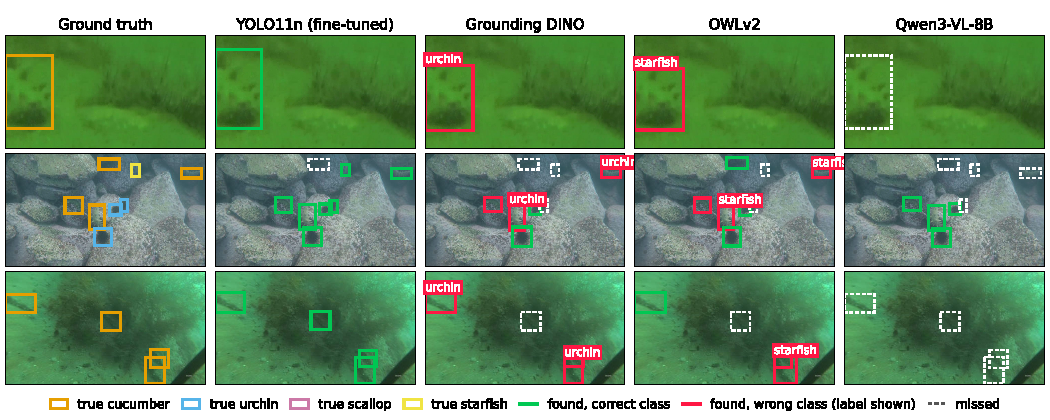
\includegraphics[width=\textwidth]{fig_examples.pdf}
\caption{Three DUO test images, cropped around their objects. The left column shows the true objects, colored by class. Every other column shows, for each true object, the model's best-overlapping box among the image's 100 highest-scoring boxes: green if the box carries the correct class, red with the assigned label if not (repeated labels on overlapping boxes are shown once), and a dashed outline if no box overlaps the object with IoU $\geq$ 0.5. This is the per-object view used in Section~\ref{sec:where}, not the output at a fixed confidence threshold. Both open-vocabulary detectors box the sea cucumbers but call them sea urchins (Grounding DINO) or starfish (OWLv2); Qwen3-VL-8B names some sea cucumbers and misses others. Images from DUO \citep{liu2021duo}, CC BY 4.0.}
\label{fig:examples}
\end{figure*}

Robots that harvest or survey benthic animals must detect each animal and know its species before acting on it. Training a detector for this requires labeled underwater images, which are costly to collect. Open-vocabulary detectors \citep{li2022glip,liu2024grounding,minderer2023scaling} and vision-language models (VLMs) that output boxes \citep{bai2025qwen25vl,bai2025qwen3vl} offer an alternative: they take the class names as text and need no task-specific training. Whether such a model can be deployed depends less on its average benchmark score than on how it fails on the classes the robot acts on, and whether those failures are visible before deployment.

Zero-shot detection is known to degrade outside web imagery \citep{robicheaux2025rf100vl}, VLM detectors recall few objects even on COCO \citep{fu2026wedetect}, and even fine-tuned underwater detectors perform unevenly across species \citep{wille2026marine}. Benchmark results are usually averages over classes, and a low score can come from missing the objects, from finding them but assigning the wrong class, or from how the model is evaluated. These causes call for different remedies before deployment.

We separate them on two established underwater benchmarks. DUO \citep{liu2021duo} contains the four seafloor animals of underwater robot-picking contests (sea cucumber, sea urchin, scallop, starfish); RUOD \citep{fu2023ruod} contains the same four and six other classes such as fish, divers and turtles. We compare six detectors fine-tuned on each benchmark with two open-vocabulary detectors (Grounding DINO, OWLv2) and three VLMs (Qwen2.5-VL-3B and -7B, Qwen3-VL-8B), and measure, beyond AP, whether each object is found, whether it is named, and how a model names an object when given the crop of its true box. Our contributions are:
\begin{itemize}
\item \textbf{Systematic mislabeling with default labels.} Given the crop of a seafloor animal, the open-vocabulary detectors rarely name it and instead give most such animals one default class. On the same images, the default changes with the class list, and re-scaling the per-class scores does not recover the classes on DUO (Section~\ref{sec:box}). This is a specific, measurable form of the label bias known for zero-shot classifiers \citep{zhao2021calibrate}, shown here for detectors on robot-relevant classes.
\item \textbf{Evaluation that conceals the failure.} On RUOD's other classes the open-vocabulary detectors reach \rOthOWL--\rOthGD{} AP, against \rOthYoloN{} for a fine-tuned YOLO11n, but on the seafloor classes, which make up all of DUO, they reach almost nothing; this class mix explains why the two benchmarks disagree, and a single average hides the failure. The VLMs fail differently: they name seafloor animals more often but find fewer of them (Sections~\ref{sec:gap}--\ref{sec:vlm}).
\item \textbf{Evaluation choices.} Output decoding, AP for VLM outputs without confidence scores, and prompt wording change scores and model rankings, consistent with observations by \citet{li2025aerialmlm} and \citet{robicheaux2025rf100vl} (Section~\ref{sec:choices}).
\end{itemize}

\section{Related Work}

\paragraph{Underwater detection benchmarks.}
DUO \citep{liu2021duo} re-annotates images from the URPC robot-picking contests and the UDD dataset \citep{liu2022udd}. RUOD \citep{fu2023ruod} contains 14,000 images with ten classes. \citet{wille2026domain} show that underwater domain factors affect both annotation quality and detector accuracy. Closest to our analysis, \citet{wille2026marine} separate localization from classification for YOLO11 on DUO and RUOD with TIDE and find scallops hardest, with foreground--background discrimination as the main problem. They study detectors trained on these benchmarks; we study models that were never trained on underwater boxes, where naming fails far more often than localization.

\paragraph{Zero-shot detection beyond web images.}
GLIP \citep{li2022glip} introduced the ODinW transfer benchmark; Grounding DINO \citep{liu2024grounding} and OWLv2 \citep{minderer2023scaling} are widely used open-vocabulary detectors. Roboflow100-VL \citep{robicheaux2025rf100vl} shows that their zero-shot AP drops sharply across 100 domains, including aquatic ones, and \citet{chhipa2024robustness} measure their robustness under distribution shifts of COCO. On aerial images, \citet{tsourveloudis2026aerial} finds that semantic confusion rather than localization limits them, based on how performance changes when the vocabulary is reduced. MarineDet \citep{liang2023marinedet} trains an open-vocabulary detector for marine objects. We measure directly, per object and with ground-truth boxes, how such detectors assign labels to classes they do not recognize, which complements the vocabulary-based evidence of \citet{tsourveloudis2026aerial}.

\paragraph{VLMs as detectors.}
Qwen2.5-VL \citep{bai2025qwen25vl} and Qwen3-VL \citep{bai2025qwen3vl} output boxes as text. \citet{fu2026wedetect} report that such models predict only part of the objects in an image, and UWBench \citep{zhang2025uwbench} evaluates VLMs on underwater understanding, including referring-expression grounding. VLM boxes carry no confidence score, so AP measures them at one operating point. \citet{li2025aerialmlm} find on aerial images that the mAP advantage of conventional detectors over multimodal language models largely comes from confidence scores, and Roboflow100-VL finds that added confidence scores and the prompt style change VLM accuracy \citep{robicheaux2025rf100vl}.

\paragraph{Error analysis.}
TIDE \citep{bolya2020tide} attributes lost AP to error types; its classification error counts misnamed boxes but does not show whether they share one wrong label, which the share of the most frequent answer does. Classifying the crops of regions is a common diagnostic of open-vocabulary recognition \citep{gu2022vild}; we apply it with ground-truth boxes. Zero-shot classifiers are known to favor some labels regardless of the input, which calibration can reduce \citep{zhao2021calibrate}; we test whether such a score offset explains the detectors' default labels.

\section{Experimental Setup}
\label{sec:setup}

\paragraph{Benchmarks.}
DUO \citep{liu2021duo} has 6,671 training and \nTestImages{} test images with \nTestObjects{} test objects of four classes: \nSeaUrchin{} sea urchins, \nStarfish{} starfish, \nSeaCucumber{} sea cucumbers and \nScallop{} scallops. RUOD \citep{fu2023ruod} has 9,800 training and \rTestImages{} test images with \rTestObjects{} test objects of ten classes: the same four seafloor classes and fish, corals, divers, cuttlefish, turtles and jellyfish. In RUOD's official split, \rDupImages{} test images (with \rDupAnn{} objects) also appear in the training set; this can only favor the fine-tuned detectors, and removing them changes their AP by at most \rDedupMax{} (e.g., \rApYoloN{} to \rDedupYoloN{} for YOLO11n). COCO AP averages over classes. The test sets are used only for final scoring.

\paragraph{Models.}
YOLOv8n \citep{jocher2023yolov8}, YOLO11n/s/m/l \citep{jocher2024yolo11} and RT-DETR-L \citep{zhao2024rtdetr} start from COCO-pretrained weights and are fine-tuned on each benchmark with one recipe (Ultralytics 8.4.60; 640-pixel input, 40 epochs, batch size 8, seed 17), selecting the checkpoint on 10\% of the training split. The zero-shot models are Grounding DINO base \citep{liu2024grounding}, OWLv2 base \citep{minderer2023scaling}, Qwen2.5-VL-3B and -7B Instruct \citep{bai2025qwen25vl} and Qwen3-VL-8B Instruct \citep{bai2025qwen3vl}, run with Hugging Face Transformers 4.57.6 \citep{wolf2020transformers}. Classes are named in plain English (``sea cucumber'' and ``sea urchin'' for holothurian and echinus). Grounding DINO receives all class names in one caption (``sea cucumber. sea urchin. scallop. starfish.'' on DUO); OWLv2 receives one query per class, ``a photo of a $\langle$class$\rangle$''. The VLMs receive the image and the prompt
\begin{quote}\small
Detect every $\langle$class list$\rangle$ in this underwater image. Answer with JSON only: a list of objects, each \{"bbox\_2d": [x1, y1, x2, y2], "label": one of [$\langle$class list$\rangle$]\}, with coordinates $\langle$coordinate phrase$\rangle$. Answer [] if there are none.
\end{quote}
with coordinates in pixels (Qwen2.5-VL) or on a 0--1000 grid (Qwen3-VL), greedy decoding and at most 1,536 new tokens; box labels are matched to the class names. On RUOD, the VLMs ran on a fixed random subset of \rSubset{} test images (seed 17), because Qwen3-VL-8B needs \secQwenVLmean{} seconds per image on average.

\paragraph{Scoring.}
We report COCO AP (IoU 0.50--0.95) with pycocotools \citep{lin2014coco}. Fine-tuned detectors keep boxes with confidence $\geq$ 0.001 (up to 300 per image), open-vocabulary detectors boxes with confidence $\geq$ 0.01. Grounding DINO is scored as in its own COCO evaluation: a class's score is the mean probability over the text tokens of its name, and the 300 best (box, class) pairs per image are kept. VLM boxes carry no score and are all scored 1.0; boxes beyond the image are clipped, and a reply cut off at the token limit is kept up to the cut. Intervals are 95\% percentile intervals from 500 bootstrap resamples of the test images \citep{efron1994introduction}; differences are computed on the same resamples. Many test images come from video footage, so they are not fully independent and the intervals are likely too narrow; we therefore rely only on large effects.

\paragraph{Per-object measures.}
An object is \emph{found} if any of the image's 100 highest-scoring boxes, of any class, overlaps it with IoU $\geq$ 0.5, and \emph{named} if such a box also carries its class. These shares do not depend on how a model ranks its boxes within the 100; on DUO, the naming failure on sea cucumbers persists when only the 10 highest-scoring boxes count or IoU $\geq$ 0.7 is required (Grounding DINO names \scNamedTopTenGD\% and \scNamedIouSeventyGD\%, OWLv2 \scNamedTopTenOWL\% and \scNamedIouSeventyOWL\%).

\paragraph{Box-crop naming test.}
To test naming without the need to find the object in the full image, each zero-shot model sees only the crop of one true box (enlarged by 10\% on each side and upscaled to at least 56 pixels on its shorter side) and must give its class. We sample up to 300 test objects per class (seed 17): \nCrops{} crops on DUO and \rCrops{} on RUOD, after dropping one degenerate 274$\times$1-pixel RUOD box. The VLMs are asked ``This underwater image shows one object. Which one is it: $\langle$class list$\rangle$? Answer with one of these names only.''; the open-vocabulary detectors still predict boxes inside the crop, and we take the class of their highest-scoring box, so for them the test does not remove localization entirely (Section~\ref{sec:box}). We report per-class accuracy and its mean over classes (chance: 25\% on DUO, 10\% on RUOD), with bootstrap intervals over crops. To change only the class list on identical images, we reran both detectors on a CPU on \vCrops{} of the DUO crops (60 per class, seed 17) with RUOD's ten class names, and Grounding DINO also with its four class names in reverse order. This CPU code gives the same answers as the GPU runs on the first \vReproCrops{} crops of each detector, with scores within \vReproDiff. These runs also record whether the winning box covers the object (IoU $\geq$ 0.5 within the crop).

\paragraph{Matched box budget.}
To compare VLMs and detectors at the same operating point, each detector keeps on every image its $k$ highest-scoring distinct boxes, where $k$ is the number of distinct boxes Qwen3-VL-8B returned there. All boxes then count equally, and we compute precision and recall at IoU $\geq$ 0.5 with the correct class. Because $k$ comes from the VLM, this favors the detectors.

\section{Results}

\begin{table*}[t]
\centering
\small
\setlength{\tabcolsep}{4.5pt}
\begin{tabular}{llccccccc}
\toprule
 & & \multicolumn{5}{c}{Full test set (\nTestImages{} images)} & First 100 images & \\
\cmidrule(lr){3-7}\cmidrule(lr){8-8}
Model & COCO AP & AP (95\% CI) & AP$_{50}$ & AR$_{100}$ & Merged AP & Sea cuc.\ AP & AP (95\% CI) & ms/image \\
\midrule
\multicolumn{9}{l}{\textit{Fine-tuned on DUO}} \\
YOLOv8n & 37.3 & 0.624 [0.593, 0.655] & 0.824 & 0.741 & 0.700 & 0.608 & 0.606 [0.482, 0.669] & 10 \\
YOLO11n & 39.5 & 0.625 [0.595, 0.652] & 0.820 & 0.747 & 0.705 & 0.606 & 0.628 [0.508, 0.692] & 11 \\
YOLO11s & 47.0 & 0.674 [0.645, 0.701] & 0.859 & 0.770 & 0.730 & 0.669 & 0.656 [0.526, 0.707] & 15 \\
YOLO11m & 51.5 & 0.685 [0.654, 0.712] & 0.857 & 0.780 & 0.742 & 0.680 & 0.684 [0.541, 0.735] & 13 \\
YOLO11l & 53.4 & 0.690 [0.662, 0.716] & 0.863 & 0.780 & 0.744 & 0.690 & 0.691 [0.556, 0.739] & 15 \\
RT-DETR-L & 53.0 & 0.669 [0.639, 0.695] & 0.849 & 0.774 & 0.718 & 0.666 & 0.692 [0.557, 0.742] & 21 \\
\midrule
\multicolumn{9}{l}{\textit{Zero-shot detectors}} \\
Grounding DINO & -- & 0.090 [0.067, 0.114] & 0.151 & 0.360 & 0.136 & 0.004 & 0.078 [0.048, 0.138] & 252$^\ddagger$ \\
OWLv2 & -- & 0.099 [0.088, 0.111] & 0.183 & 0.190 & 0.151 & 0.001 & 0.107 [0.078, 0.140] & 328 \\
\midrule
\multicolumn{9}{l}{\textit{Zero-shot VLMs}} \\
Qwen2.5-VL-3B & -- & 0.000 [0.000, 0.000] & 0.000 & 0.000 & 0.000 & 0.000 & 0.000 [0.000, 0.000] & 200 \\
Qwen2.5-VL-7B & -- & 0.013 [0.009, 0.018] & 0.024 & 0.021 & 0.016 & 0.004 & 0.018 [0.006, 0.034] & 632 \\
Qwen3-VL-8B & -- & \multicolumn{5}{c}{not run on the full test set} & 0.054 [0.043, 0.087] & 15{,}918 \\
\bottomrule
\end{tabular}
\caption{Detection results on the DUO test set (COCO protocol, pycocotools). Intervals are 95\% paired bootstrap intervals over test images. COCO AP is the published value for the fine-tuned architectures (Ultralytics). Merged AP treats all four classes as one, so a box counts regardless of its label. Qwen3-VL-8B was run only on the first 100 test images; the last column compares all models on those images. VLM boxes carry no confidence score and are all scored 1.0. Time per image on one RTX 5090: for the fine-tuned detectors, the median over 200 test images processed one at a time on an idle GPU, including pre- and post-processing; for the zero-shot models, wall-clock time over the whole run, including image loading. $^\ddagger$Grounding DINO shared the GPU with another job, so its time is an upper bound. Qwen2.5-VL is fast because it mostly returns an empty answer.}
\label{tab:main}
\end{table*}


\subsection{The Two Benchmarks Disagree}
\label{sec:gap}

On DUO, every zero-shot model is far below every fine-tuned detector (Table~\ref{tab:main}): the best zero-shot model, OWLv2, reaches \apOWL{} AP, the weakest fine-tuned detector \apYoloEightN, a gap of \dGap{} \dciGap. On RUOD the gap is much smaller: \rGapWeakest{} reaches \rApWeakest{} and \rGapBest{} \rApGD, a gap of \rdGap{} \rdciGap, and Qwen3-VL-8B reaches \rApQwenVL{} on the VLM subset. The difference lies in the classes. On RUOD's six other classes, the open-vocabulary detectors reach \rOthGD{} \rOthciGD{} (Grounding DINO) and \rOthOWL{} \rOthciOWL{} (OWLv2), against \rOthYoloN{} for YOLO11n; on its four seafloor classes they reach \rSeaGD{} \rSeaciGD{} and \rSeaOWL{} \rSeaciOWL, against \rSeaYoloN{} for YOLO11n. Qwen3-VL-8B shows the same split (\rOthQwenVL{} against \rSeaQwenVL). The seafloor classes are also harder for the fine-tuned detectors, but much less so. DUO consists only of these four classes, so its average shows the zero-shot failure in full, while RUOD's average dilutes it with classes that the zero-shot models handle reasonably well.

\subsection{Found but Misnamed}
\label{sec:where}

\begin{table*}[t]
\centering
\small
\setlength{\tabcolsep}{2.7pt}
\begin{tabular}{lcccccccll}
\toprule
 & \multicolumn{2}{c}{DUO, full images} & \multicolumn{2}{c}{RUOD seafloor, full} & \multicolumn{3}{c}{Named, box crop} & \multicolumn{2}{c}{Default answer, seafloor crops} \\
\cmidrule(lr){2-3}\cmidrule(lr){4-5}\cmidrule(lr){6-8}\cmidrule(lr){9-10}
Model & Found & Named & Found & Named & DUO & RUOD sea. & RUOD other & DUO & RUOD \\
\midrule
YOLO11n (fine-tuned) & 96 & 95 & 95 & 94 & -- & -- & -- & -- & -- \\
\midrule
Grounding DINO & 69 & 59 & 73 & 18 & 28 & 1 & 59 & sea urchin 95\% & fish 76\% \\
\quad Latin names & -- & -- & -- & -- & 28 & 2 & 59 & holothurian 88\% & fish 77\% \\
OWLv2 & 62 & 50 & 76 & 22 & 26 & 4 & 70 & starfish 91\% & jellyfish 65\% \\
\quad Latin names & -- & -- & -- & -- & 28 & 4 & 70 & starfish 65\% & jellyfish 60\% \\
\midrule
Qwen2.5-VL-3B & 0 & 0 & 0 & 0 & 33 & 34 & 64 & sea urchin 57\% & sea urchin 73\% \\
Qwen2.5-VL-7B & 3 & 3 & 8 & 6 & 33 & 36 & 76 & sea cucumber 59\% & sea cucumber 54\% \\
Qwen3-VL-8B & 44 & 41 & 41 & 38 & 48 & 48 & 87 & sea cucumber 52\% & sea cucumber 45\% \\
\bottomrule
\end{tabular}
\caption{Finding and naming (\%). Found: share of true objects overlapped (IoU $\geq$ 0.5) by any of the image's 100 highest-scoring boxes, of any class; named: by such a box with the correct class (DUO: all objects; RUOD: the four seafloor classes; VLMs on RUOD: the \rSubset-image subset). Named, box crop: mean per-class accuracy when the model sees only the crop of a true box (chance 25\% on DUO, 10\% on RUOD; RUOD columns averaged over the four seafloor and the six other classes). Default answer: the answer a model gives most often for seafloor crops, and the share of seafloor crops that receive it. YOLO11n was not run on crops.}
\label{tab:naming}
\end{table*}


The open-vocabulary detectors put boxes on many seafloor animals but rarely give them the right class (Table~\ref{tab:naming}, Figure~\ref{fig:examples}). On DUO, Grounding DINO finds \foundGD\% of all objects and names \namedGD\%; for sea cucumbers it finds \scFoundGD\% and names \scNamedGD\%, labeling \scUrchinGD{} of the \scFoundNGD{} it finds as sea urchins. OWLv2 finds \scFoundOWL\% of the sea cucumbers and names \scNamedOWL\%, labeling \scStarOWL{} of \scFoundNOWL{} as starfish. On RUOD's seafloor classes, Grounding DINO finds \rFoundSeaGD\% and names \rNamedSeaGD\%; OWLv2 finds \rFoundSeaOWL\% and names \rNamedSeaOWL\%. The fine-tuned YOLO11n finds \foundYoloN\% of DUO's objects and names \namedYoloN\%, so the images contain the information needed. Localization is weaker as well: merged-class AP, which ignores labels, is \mgGD{} and \mgOWL{} for the two detectors on DUO, against \mgYoloEightN--\mgYoloL{} for the fine-tuned detectors.

\subsection{Naming the Box Crop: Default Labels}
\label{sec:box}

\begin{figure*}[t]
\centering
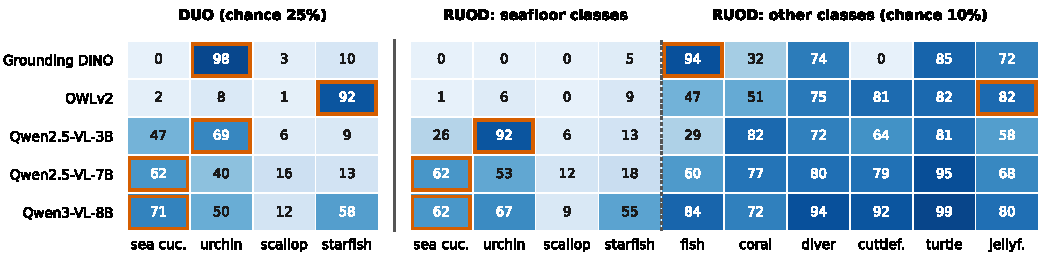
\includegraphics[width=\textwidth]{fig_heatmap.pdf}
\caption{Box-crop naming test: share of crops (\%) named correctly when a model sees only the crop of a true box, per class, on DUO and RUOD. Outlined cells mark each model's default answer, the class it gives most often to seafloor crops; high accuracy in these cells reflects the default rather than recognition. All 95\% intervals are within $\pm$\cropMaxHalf{} percentage points.}
\label{fig:heatmap}
\end{figure*}

The box-crop test removes the need to find the object in the full image (Figure~\ref{fig:heatmap}, Table~\ref{tab:naming}). On RUOD, both open-vocabulary detectors name the six other classes well, \rCropOthGD\% \rCropOthciGD{} (Grounding DINO) and \rCropOthOWL\% \rCropOthciOWL{} (OWLv2) on average, but name only \rCropSeaGD\% \rCropSeaciGD{} and \rCropSeaOWL\% \rCropSeaciOWL{} of the seafloor crops correctly. They do not spread their errors over the classes. Grounding DINO gives \dlRuodGD\% \dlRuodciGD{} of RUOD's seafloor crops the answer ``\dlRuodLabGD'', and OWLv2 gives \dlRuodOWL\% \dlRuodciOWL{} the answer ``\dlRuodLabOWL''. On DUO, whose class list has no fish or jellyfish, the defaults are ``\dlDuoLabGD'' (\dlDuoGD\% of the crops) and ``\dlDuoLabOWL'' (\dlDuoOWL\%). This comparison changes both the images and the class list, so we also changed only the class list on the same DUO crops. With the Latin names ``holothurian'' and ``echinus'', Grounding DINO's default becomes ``\dlDuoLabGDlatin'' (\dlDuoGDlatin\%), and its accuracy on sea urchins falls from \cropUrchGD\% to \cropUrchGDlatin\%. With RUOD's ten class names on \vCrops{} of the same DUO crops, Grounding DINO's default moves from ``\vTopLabGDfour'' (\vTopGDfour\% of these crops) to ``\vTopLabGDten'' (\vTopGDten\% \vTopciGDten) and OWLv2's from ``\vTopLabOWLfour'' (\vTopOWLfour\%) to ``\vTopLabOWLten'' (\vTopOWLten\% \vTopciOWLten), and mean accuracy over the four true classes falls to \vAccGDten\% and \vAccOWLten\%. Reversing the order of the four names in Grounding DINO's caption gives the same answer on \vRevSame{} of \vRevN{} crops, so its default follows the name, not its position.
These runs also show that a detector's highest-scoring box in a crop is often not on the animal. With RUOD's names, Grounding DINO's box covers the object in \vCovGDten\% \vCovciGDten{} of the crops and OWLv2's in \vCovOWLten\% \vCovciOWLten, and most other boxes barely overlap it; with the four DUO names, Grounding DINO's box covers the object in \vCovGDrev\% of the crops, and \vCovTopGDrev\% of those are called ``sea urchin''. Where the box does cover the animal, the default also remains with RUOD's names: Grounding DINO calls \vCovTopGDten\% of these crops ``fish'' and names \vCovCorGDten\% correctly, and OWLv2 calls \vCovTopOWLten\% ``jellyfish'' and names \vCovCorOWLten\% correctly.
The default therefore depends on the class list, not only on the animal, and a default class can look well recognized: Grounding DINO's \cropUrchGD\% on DUO's sea urchins and \rCropFishGD\% on RUOD's fish are inflated by its default. The mean accuracy over classes, which a constant answer cannot raise above chance, is \cropGD\% and \cropOWL\% on DUO (chance 25\%). A constant per-class score offset does not explain the defaults. Standardizing each class's crop scores over all crops of a benchmark, which uses test-set statistics and therefore favors this correction, breaks up Grounding DINO's default on DUO (its most frequent answer falls from \dlDuoGD\% to \calDuoTopGD\% of the crops) but leaves mean accuracy at chance (\calDuoRawGD\% to \calDuoGD\% \calDuociGD; OWLv2 \calDuoRawOWL\% to \calDuoOWL\%). On RUOD it raises Grounding DINO's seafloor accuracy from \calRuodRawGD\% to \calRuodGD\% \calRuodciGD, so part of its ``fish'' default is a score offset, but OWLv2's only from \calRuodRawOWL\% to \calRuodOWL\%, while its accuracy on the other classes drops from \calRuodOthRawOWL\% to \calRuodOthOWL\%. The failure does not come from small objects: on RUOD seafloor crops at least 150 pixels on the shorter side, Grounding DINO is correct on \rBigSeaGD\% and OWLv2 on \rBigSeaOWL\%, against \rBigOthGD\% and \rBigOthOWL\% for other classes of that size.

\subsection{VLMs Name More but Find Less}
\label{sec:vlm}

The VLMs name seafloor animals far more often in the box-crop test: Qwen3-VL-8B names \rCropSeaQwenVL\% \rCropSeaciQwenVL{} of RUOD's seafloor crops and has a mean accuracy of \cropQwenVL\% on DUO, \cropdGD{} percentage points \cropdciGD{} above Grounding DINO. They also lean toward one answer (Qwen3-VL-8B gives ``\dlRuodLabQwenVL'' to \dlRuodQwenVL\% of RUOD's seafloor crops), but much less. In full images, however, Qwen3-VL-8B finds only \foundQwenVL\% of DUO's objects and \scFoundQwenVL\% of its sea cucumbers, against \foundGD\% and \scFoundGD\% for Grounding DINO; on RUOD's seafloor classes it finds \rFoundSeaQwenVL\%. Its main failure is finding the objects, the opposite of the open-vocabulary detectors. Qwen2.5-VL-7B finds even fewer, partly because it answers with an empty list on \pctEmptyQSeven\% of DUO's images (Section~\ref{sec:choices}). Scallops are hard for every model: none names more than \rCropScalMax\% of RUOD's scallop crops.

\subsection{Evaluation Choices Change the Verdict}
\label{sec:choices}

\begin{table}[t]
\centering
\small
\setlength{\tabcolsep}{3pt}
\begin{tabular}{lc}
\toprule
Setting & Value (95\% CI) \\
\midrule
\multicolumn{2}{l}{\textit{(a) Grounding DINO decoding (DUO AP)}} \\
Own scoring $-$ phrase decoding & +0.042 [0.032, 0.053] \\
OWLv2 $-$ Grounding DINO & +0.009 [$-$0.015, 0.031] \\
\midrule
\multicolumn{2}{l}{\textit{(b) VLM prompt, $\Delta$AP on DUO (first 100 images)}} \\
\multicolumn{2}{l}{\quad no ``Answer []'' / one class per prompt:} \\
\quad Qwen2.5-VL-3B & +0.017 / +0.000 \\
\quad Qwen2.5-VL-7B & +0.000 / +0.018 \\
\quad Qwen3-VL-8B & $-$0.006 / +0.010 \\
\midrule
\multicolumn{2}{l}{\textit{(c) Qwen3-VL-8B minus Grounding DINO}} \\
DUO AP & $-$0.043 [$-$0.064, $-$0.016] \\
DUO P / R, matched boxes & +0.112 / +0.130 \\
RUOD AP (subset) & $-$0.061 [$-$0.070, $-$0.036] \\
RUOD P / R, matched boxes & +0.177 / +0.226 \\
\midrule
\multicolumn{2}{l}{\textit{(d) Qwen3-VL-8B minus OWLv2}} \\
DUO AP & $-$0.051 [$-$0.061, $-$0.040] \\
DUO P / R, matched boxes & $-$0.001 / +0.061 \\
RUOD AP (subset) & $-$0.009 [$-$0.019, 0.017] \\
RUOD P / R, matched boxes & +0.121 / +0.155 \\
\bottomrule
\end{tabular}
\caption{Evaluation choices. (a) The same Grounding DINO outputs scored as in its own COCO evaluation or through phrase decoding. (b) Change in AP when the sentence ``Answer [] if there are none'' is removed, or when the four classes are asked for one at a time (intervals in the text). (c, d) P, R: precision and recall. At a matched box budget (each detector keeps as many boxes per image as the VLM returned, all counting equally; IoU $\geq$ 0.5, correct class) the VLM matches or exceeds them; at IoU $\geq$ 0.75 its advantage shrinks (Section~\ref{sec:choices}). Differences are Qwen3-VL-8B minus the detector.}
\label{tab:choices}
\end{table}


\paragraph{Output decoding.}
The Hugging Face pipeline turns each Grounding DINO box into a text phrase that must be matched to a class name; on DUO, \pctUnmatchedText\% of the phrases match no class (e.g.\ ``seachin'', a fragment of ``sea urchin''), and those boxes are lost. Scoring the same outputs as in Grounding DINO's own evaluation raises AP from \apGDtext{} to \apGD{} (Table~\ref{tab:choices}a), more than the difference between OWLv2 and Grounding DINO.

\paragraph{VLM outputs without confidence scores.}
AP ranks Qwen3-VL-8B below Grounding DINO on both benchmarks, below OWLv2 on DUO and level with it on RUOD (Table~\ref{tab:choices}c,d). At a matched box budget the ranking changes: on DUO, Qwen3-VL-8B exceeds Grounding DINO in precision (\bdPGD{} \bdciPGD) and recall (\bdRGD{} \bdciRGD), and matches OWLv2 in precision while exceeding it in recall (\bdROWL{} \bdciROWL); on RUOD it exceeds both detectors in precision and recall, for example Grounding DINO by \rbdPGD{} \rbdciPGD{} and \rbdRGD{} \rbdciRGD. AP, however, also rewards tight boxes. At IoU $\geq$ 0.75 on DUO, Qwen3-VL-8B's advantage over Grounding DINO shrinks to \btdPGD{} \btdciPGD{} in precision and \btdRGD{} \btdciRGD{} in recall, and it falls below OWLv2 in precision (\btdPOWL{} \btdciPOWL): only \keepTightQwenVL\% of its correct boxes at IoU 0.5 also reach 0.75, against \keepTightGD\% for Grounding DINO, \keepTightOWL\% for OWLv2 and \keepTightYoloN\% for YOLO11n. The VLM's lower AP thus comes partly from its missing confidence ranking, as \citet{li2025aerialmlm} observed on aerial images, and partly from looser boxes.

\paragraph{Prompt wording.}
With ``Answer [] if there are none'' in the prompt, Qwen2.5-VL-3B returns an empty list on \nEmptyQThree{} of \nRepQThree{} DUO test images and Qwen2.5-VL-7B on \nEmptyQSeven, although \nImagesWithObjects{} images contain objects. Without the sentence (first 100 images) neither returns an empty list, yet AP barely changes (Table~\ref{tab:choices}b; 7B: \dPromptSeven{} \dciPromptSeven). Asking for one class per prompt, which Roboflow100-VL found better for Qwen2.5-VL, raises AP slightly for the 7B model (\dSingleSeven{} \dciSingleSeven) and not significantly for Qwen3-VL-8B (\dSingleQwen{} \dciSingleQwen). Neither change brings any VLM close to the fine-tuned detectors.

\paragraph{What does not explain the gap.}
Halving the image-pixel budget of Qwen2.5-VL-7B changes its DUO AP by \dResolution{} \dciResolution. Latin class names do not improve either detector on DUO (Grounding DINO, common minus Latin: \dLatinGd{} \dciLatinGd) and leave their RUOD crop accuracy unchanged (\rCropGD\% and \rCropOWL\% mean accuracy with common names, \rCropGDlatin\% and \rCropOWLlatin\% with Latin names).

\section{Discussion}
\label{sec:discussion}

\paragraph{Implications for deployment.}
A picking robot acts on the class. Current zero-shot detectors can propose where many seafloor animals are, but assign them a default class; a robot relying on them would act on the wrong class for most sea cucumbers. This failure is systematic rather than random, so it does not average out over repeated views, and which class absorbs the errors changes when the class list is edited, for example when a new target class is added. The VLMs name these animals better but miss many and need \secQwenVLmean{} s per image, against \msYoloMin--\msYoloMax{} ms for the fine-tuned detectors (Table~\ref{tab:main}). Combining zero-shot boxes with a VLM or a classifier trained on a few labeled examples for naming is a natural next step that we have not tested. We did not run any model on a robot; our conclusions concern the perception step and the tests that should precede deployment.

\paragraph{Implications for evaluation.}
A benchmark average can hide a failure on the classes that matter: zero-shot detection looks moderately useful on RUOD and useless on DUO, yet both benchmarks show the same failure on the same four classes. All of the following checks need only a labeled test set and can be run before deployment: per-class AP for the target classes; per-object found and named shares; naming accuracy given the true box together with the share of the most frequent answer, which exposes default labels; the same test with an edited class list; the decoding path; and, for VLMs, confidence-free comparisons at more than one IoU threshold, and the prompt.

\paragraph{Limitations.}
In RUOD, only \rMixedImages{} of the \rSeaImages{} test images with seafloor animals contain any other class, so the seafloor classes and their imaging conditions cannot be separated: we cannot tell whether the failure stems from the animals or from the murky seafloor footage they appear in. Two observations argue against image quality as the whole explanation: on DUO's seafloor footage, the fine-tuned YOLO11n names \namedOfFoundMinYoloN--\namedOfFoundMaxYoloN\% of the objects it finds in each class, and Qwen3-VL-8B names \rCropSeaQwenVL\% of RUOD's seafloor crops. The default-label finding holds either way. Many test images are frames of the same videos, and several crops can come from one image, so our bootstrap intervals, which treat images or crops as independent, are likely too narrow; we draw conclusions only from large effects. The calibration control uses test-set statistics, and the class-list changes on identical crops cover a few lists, two detectors and \vCrops{} crops. We test two open-vocabulary detectors and one prompt template per model, apart from the variations in Section~\ref{sec:choices}; other prompts, thresholds or detectors may behave differently. The VLMs ran on a \rSubset-image subset of RUOD, the box-crop test removes context around each object, the open-vocabulary detectors' best box in a crop often misses the animal, so their crop accuracy mixes naming with localization, and the shared word ``sea'' in two DUO class names may contribute to Grounding DINO's default there. We did not check DUO's split for duplicate images, and underwater annotations are imperfect \citep{wille2026domain}.

\section{Conclusion}

On two established underwater benchmarks, zero-shot open-vocabulary detectors and VLMs handle several underwater classes but fail on the four seafloor animals that underwater picking robots target. The open-vocabulary detectors place boxes on many of these animals but, even given the crop of the true box, give most of them one default class that changes with the class list and is not removed by re-scaling class scores. The VLMs name these animals more often but find fewer of them and draw looser boxes. Because DUO contains only these classes and RUOD mixes them with others, the two benchmarks give very different impressions of the same failure. Before zero-shot perception is deployed on a robot, it should be tested with per-class, per-object and box-given measures alongside AP.

\bibliography{references}

\end{document}
